The previous section overviewed the samples that are reconstructed using basic requirements laid out in \Cref{sec:tag_reconstruction,sec:gamma_reconstruction}.
In this section concrete selections will be discussed that will lead to background suppression and a best photon candidate
and best tag-candidate selection.

\subsection{Primary photon candidate selection}\label{sec:primary_photon_candidate_selection}
Contrary to the tag side, a selection of the the best photon candidate in the range $\EB>1.4~\gev$ is effectively trivial based on the discussion in \Cref{sec:event_reconstruction}.
As for 99.7\% and 99.8\% of the signal \MC sample the highest \EB photon is the correct photon originating from \BtoXsgamma decay,
this is chosen as then best photon-candidate requirement with virtually no signal efficiency loss.
Judging from \Cref{fig:photon_reco_candidates}, this provides an approximately 3\% background suppression.
For the rest of the thesis, this selection on photon candidates will always implied in figures and calculations.
\subsection{Main photon backgroundes sources}\label{sec:main_background_sources}

Based on \Cref{fig:spectrum_after_reco}, number of photon and tag candidates originating 
in non-\BB events is significantly larger than number of \B meson events.
The proportion of \qqbar to \BB event candidates is 92.5\% to 7.5\% for \FEI \Bp mode;
and 91.7\% to 8.3\% for \FEI \Bz.

The majority of background photon candidates originate in $\piz\ra\g\g$ or $\eta\ra\g\g$ decays.
This in total accounts for roughly 85\% of background photon candidates.
Photon candidates, broken down by their mother-particle, are shown in \Cref{fig:photon_sources}.
Other sources, such as initial-state radiation, neutron annihilation, parton-shower final-state radation, $\omega(782)$, $\eta'$ decays (in decreasing order) individually make up between 0.5\%-3\% of sample.
All other sources individually make up less than 0.5\% and include various hadron decays that are produced in continuum or \B events.
The backgrounds are similar for both \FEI \Bp and \Bz modes.
Note that some photon candidates can be misidentified, in particular XXXXX.

The reason why $\piz\ra\g\g$ and $\eta\ra\g\g$ decays are such a prominent background is related to the fact that they can often be produced in hadronic decays and tend to decay asymmetrically -- where one photon has a much larger energy than the other.
The hadronic decay, overall, mimics the hadronised $X_s$ system, whereas the high-energy photon is taken as the high-energy photon candidate, therefore resulting is similar kinematics.
However, for \B decays, this background drops off rapidly with photon energy, and at high-\EB becomes negligibly small because processes producing photons with $\EB\approx m_B/2$ in \B decays are rare.
No such constraint exist for continuum events where light-hadrons can be created in large numbers.
Therefore, \piz and \eta suppression, while important for \B decays, also highly coincides with continuum event suppression.

\begin{figure}[htbp!]
    \centering
    \subcaptionbox{\label{fig:bp_photon_sources}}{
        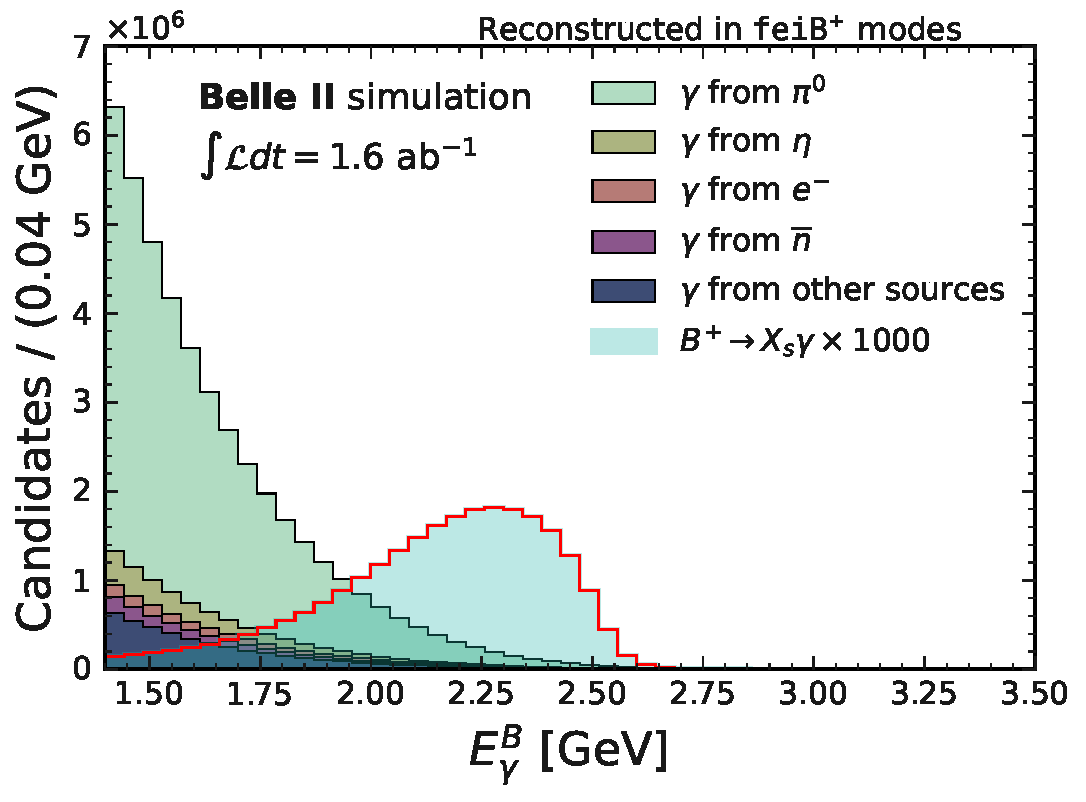
\includegraphics[width=0.395\textwidth]{figures/event_selection/Bp_photon_sources.pdf}
    }
    \subcaptionbox{\label{fig:bz_photon_sources}}{
        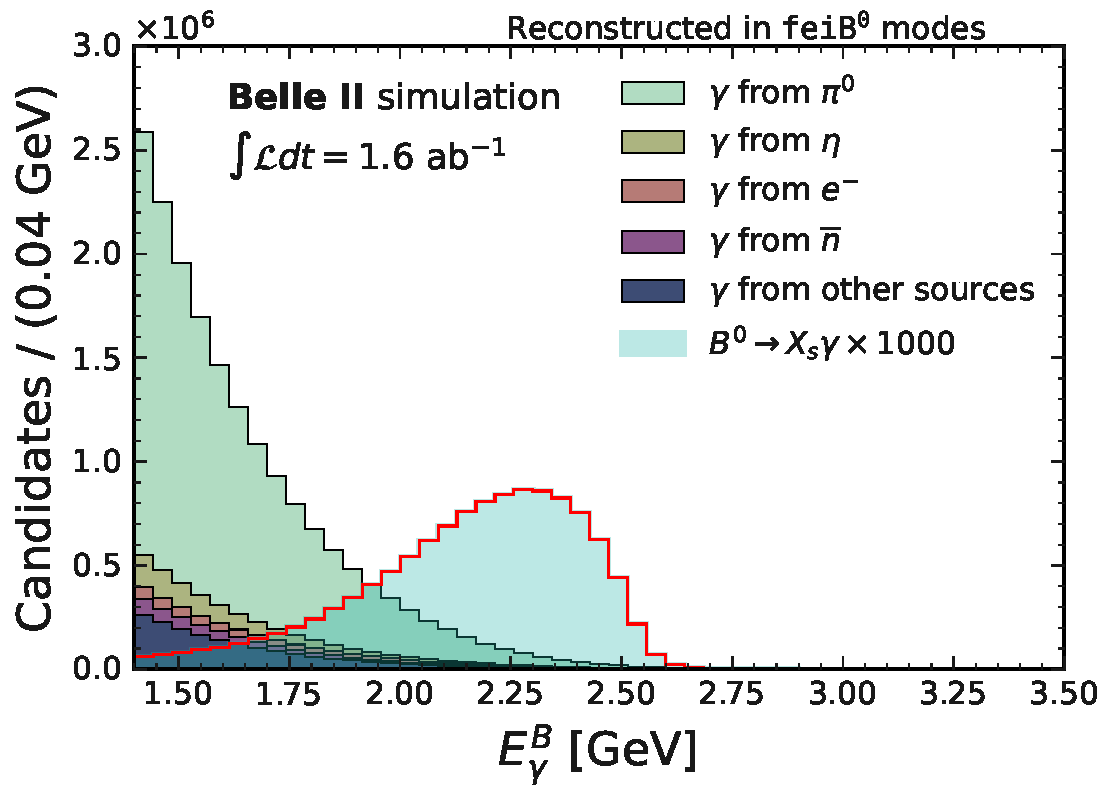
\includegraphics[width=0.395\textwidth]{figures/event_selection/Bz_photon_sources.pdf}
        }
    \caption{\label{fig:photon_sources} The background photon distribution after reconstruction, stacked by the photon mother-particle species.
    A scaled \BtoXsgamma spectrum is also overlaid.
    Only one photon candidate per event is shown, but at this stage it may still be paired with multiple tag-side candidates.
    Roughly 85\% of candidates originate in \pi\ra\g\g or \eta\ra\g\g decays.
    Other important backgrounds are photons from initial-state radiation and bremmstrahlung; and neutron-annihilation processes.
    These account for approximately 3\% each.
    The leftover 10\% originate in various other decays.}
\end{figure}

At this stage, \BtoXsgamma events make up 0.05\% of the \FEI \Bp sample and 0.07\% of the \FEI \Bz sample.
To reduce the discussed background components the following strategy is adopted:
\begin{itemize}
    \item Suppress misidentified photons (different particle species);
    \item Suppress $\piz\ra\g\g$ and $\eta\ra\g\g$ decays;
    \item Suppress \epem\ra\qqbar events;
    \item Reoptimise all selections simultaneously to adopt a final set of selections.
\end{itemize}

\subsection{Misidentified photon suppression}\label{sec:selection_clusZMVA}

